% настройки в preamble.inc
\documentclass[14pt]{extarticle}

\usepackage[russian]{babel}
\usepackage[utf8]{inputenc}
\usepackage[T2A]{fontenc}

\usepackage{graphicx}  
\usepackage{amsfonts}
\usepackage{amsmath}
\usepackage{amssymb}
\usepackage{mathtools}
\usepackage{upgreek}
\usepackage{xfrac}


\usepackage{listings}

\lstset{
	captionpos=t,
	breaklines=true,         % автоматически переносить строки 
	breakatwhitespace=false, % переносить строки по пробелу
	%backgroundcolor=\color{mylightgray},rulecolor=\color{red},  % choose the background color; you must add \usepackage{color} or \usepackage{xcolor}; should come as last argument
	basicstyle=\footnotesize\ttfamily,        % the size of the fonts that are used for the code
	breakatwhitespace=false,         % sets if automatic breaks should only happen at whitespace
	breaklines=true,                 % sets automatic line breaking
	captionpos=t,                    % sets the caption-position to bottom
	commentstyle=\color{green},    % comment style
	extendedchars=false,              % lets you use non-ASCII characters; for 8-bits encodings only, does not work with UTF-8
	firstnumber=0,                % start line enumeration with line 1000
	frame=single,
	%rulesepcolor=\color{green},	                   % adds a frame around the code
	keepspaces=true,                 % keeps spaces in text, useful for keeping indentation of code (possibly needs columns=flexible)
	keywordstyle=\color{blue}\textbf,       % keyword style
	language=python,                 % the language of the code
	morekeywords={*,...},            % if you want to add more keywords to the set
	numbers=left,                    % where to put the line-numbers; possible values are (none, left, right)
	numbersep=5pt,                   % how far the line-numbers are from the code
	%numberstyle=\scriptsize\color{mygray}, % the style that is used for the line-numbers
	rulecolor=\color{black},         % if not set, the frame-color may be changed on line-breaks within not-black text (e.g. comments (green here))
	showspaces=false,                % show spaces everywhere adding particular underscores; it overrides 'showstringspaces'
	showstringspaces=false,          % underline spaces within strings only
	showtabs=false,                  % show tabs within strings adding particular underscores
	stepnumber=1,                    % the step between two line-numbers. If it's 1, each line will be numbered
	%stringstyle=\color{mymauve},     % string literal style
	tabsize=4,	                   % sets default tabsize to 2 spaces
	%title=\lstname                   % show the filename of files included with \lstinputlisting; also try caption instead of title
}

\lstset{
	captionpos=t,
	breaklines=true,         % автоматически переносить строки 
	breakatwhitespace=false, % переносить строки по пробелу
	%backgroundcolor=\color{mylightgray},rulecolor=\color{red},  % choose the background color; you must add \usepackage{color} or \usepackage{xcolor}; should come as last argument
	basicstyle=\footnotesize\ttfamily,        % the size of the fonts that are used for the code
	breakatwhitespace=false,         % sets if automatic breaks should only happen at whitespace
	breaklines=true,                 % sets automatic line breaking
	captionpos=t,                    % sets the caption-position to bottom
	commentstyle=\color{green},    % comment style
	extendedchars=false,              % lets you use non-ASCII characters; for 8-bits encodings only, does not work with UTF-8
	firstnumber=0,                % start line enumeration with line 1000
	frame=single,
	%rulesepcolor=\color{green},	                   % adds a frame around the code
	keepspaces=true,                 % keeps spaces in text, useful for keeping indentation of code (possibly needs columns=flexible)
	keywordstyle=\color{blue}\textbf,       % keyword style
	language=SQL,                 % the language of the code
	morekeywords={*,...},            % if you want to add more keywords to the set
	numbers=left,                    % where to put the line-numbers; possible values are (none, left, right)
	numbersep=5pt,                   % how far the line-numbers are from the code
	%numberstyle=\scriptsize\color{mygray}, % the style that is used for the line-numbers
	rulecolor=\color{black},         % if not set, the frame-color may be changed on line-breaks within not-black text (e.g. comments (green here))
	showspaces=false,                % show spaces everywhere adding particular underscores; it overrides 'showstringspaces'
	showstringspaces=false,          % underline spaces within strings only
	showtabs=false,                  % show tabs within strings adding particular underscores
	stepnumber=1,                    % the step between two line-numbers. If it's 1, each line will be numbered
	%stringstyle=\color{mymauve},     % string literal style
	tabsize=4,	                   % sets default tabsize to 2 spaces
	%title=\lstname                   % show the filename of files included with \lstinputlisting; also try caption instead of title
}


\usepackage{enumerate}
%\usepackage{multirow}
%\usepackage{tikz}
%\usetikzlibrary{arrows,positioning,shadows}
%\usepackage{paralist,array}

\usepackage{geometry}
\geometry{right=20mm}
\geometry{left=30mm}
\geometry{bottom=20mm}
\geometry{ignorefoot}% считать от нижней границы текста

\setlength{\parindent}{1.25 cm}
\setlength{\parskip}{1ex}
\renewcommand{\baselinestretch}{1.5}

\usepackage[toc,page]{appendix}

\usepackage{titlesec}
\titleformat{\section}
  {\normalfont\fontsize{14}{14}\bfseries}{\thesection}{1em}{}
\titleformat{\subsection}
  {\normalfont\fontsize{14}{14}\bfseries}{\thesubsection}{1em}{}

\usepackage[intoc]{nomencl}
\renewcommand{\nomname}{Обозначения и сокращения}
\makenomenclature

%Подписи
\usepackage		[margin		= 10	pt,
%					font		= footnotesize, 
					labelfont	= bf, 
					labelsep	= endash, 
					labelfont	= bf,
%					textfont	= sl,
					margin		= 0 	pt,  
					aboveskip 	= 4		pt, 
					belowskip 	= -6	pt,
					figurename= Рисунок] {caption}
\usepackage		[margin		= 10	pt,
					font		= footnotesize, 
					labelfont	= bf, 
					labelsep	= endash, 
					labelfont	= bf,
					textfont	= sl,
					margin		= 0 	pt,  
					aboveskip 	= 4		pt, 
					belowskip 	= 6	pt]	{subcaption}


\newcommand\Referat{%реферат
	\chapter*{Реферат}%
}

\addto\captionsrussian{%
	\def\contentsname{%
		Содержание}%
	\def\bibname{%
		Список~
		использованных~
		источников}%
}


\usepackage{enumitem}
\usepackage{kosrem}
\usepackage{gensymb}
%\usepackage{tempora}

\begin{document}




\setcounter{page}{3}

% СОДЕРЖАНИЕ 
\clearpage
\tableofcontents

% ВВЕДЕНИЕ
\clearpage
\section*{Введение}
\addcontentsline{toc}{section}{Введение}
В наше время тяжело представить медиапространство без фильмов. Современным зрителям становится все тяжелее и тяжелее подобрать киноленту, что их завлечет и понравится. Следовательно, для желающих посмотреть интересное для них кино требуется нечто, способное порекомендовать удовлетворяющую запросы ленту. Приложение для рекомендации фильмов способно решить данный вопрос.
   
Целью данной работы является реализация простого в использовании и многофункционального приложения для получения информации о фильмах и их рекомендации пользователю.

Для достижения поставленной цели необходимо решить следующие задачи:
\begin{itemize}
	\item[1)] формализовать задание, выделив соответствующих пользователей и их функционал;
	\item[2)] провести анализ существующих решений;
	\item[3)] провести анализ СУБД и выбрать наиболее подходящую;
	\item[4)] спроектировать базу данных;
	\item[5)] спроектировать архитектуру приложения;
	\item[6)] разработать приложение.
\end{itemize}

% АНАЛИТИЧЕСКАЯ ЧАСТЬ
\clearpage
\section{Аналитический раздел}
В данном разделе будет поставлена задача, рассмотрены возможные пользователи системы, модели данных и СУБД.

\subsection{Постановка задачи}
Разработать программу, предоставляющую интерфейс для получения информации о фильмах, рекомендованных пользователю.  Посредством интерфейса нужно обеспечить для пользователя выбор любимых жанров и актёров, доступ к списку рекомендованных фильмов с информацией о них.

\subsection{Пользователи системы}
В системе существуют следующие виды пользователей:
\begin{itemize}
	\item[1)] гость;
	\item[2)] авторизованный пользователь;
	\item[3)] администратор.
	
\end{itemize}

\subsubsection{Гость}
Гость — это неавторизованный пользователь, обладающий минимальным набором возможностей взаимодействия с системой. Он может авторизоваться, просмотреть общий список фильмов, актеров, жанров с информацией о них.
\subsubsection{Авторизованный пользователь}
В функционал авторизованного пользователя входит возможность просмотра общего списка фильмов, актеров, жанров с информацией о них. Также есть возможность выбрать любимые жанры и актеров. Помимо этого пользователь может получить список рекомендуемых ему фильмов, основанных на выборе любимых актеров и жанров.
\subsubsection{Администратор}
Администратор - это пользователь, обладающий возможностью просмотра, добавления, удаления данных, связанных с фильмами актерами, жанрами, студиями, режиссерами, пользователями.

\subsection{Анализ существующих решений}
В настоящее время существует множество популярных медиа-сервисов, как для фильмов, так и для музыки. Рассмотрим некоторые из них.

\subsubsection{Кино-сервисы}
Сейчас появилось очень много сервисов для просмотра фильмов: <<Кинопоиск>>, <<Ivi>>, <<Netflix>>  и другие. На них можно смотреть фильмы и сериалы, но система рекомендаций есть на всех из них. Тот же <<Кинопоиск>> лишь недавно вновь вернул раздел рекомендаций на своем сайте. Рекомендации основаны на оценках фильмов пользователем. Ниже на Рисунке \ref{img:kinopoisk} продемонстрирован внешний вид данного раздела.

\begin{figure}[h!]
	\centering
	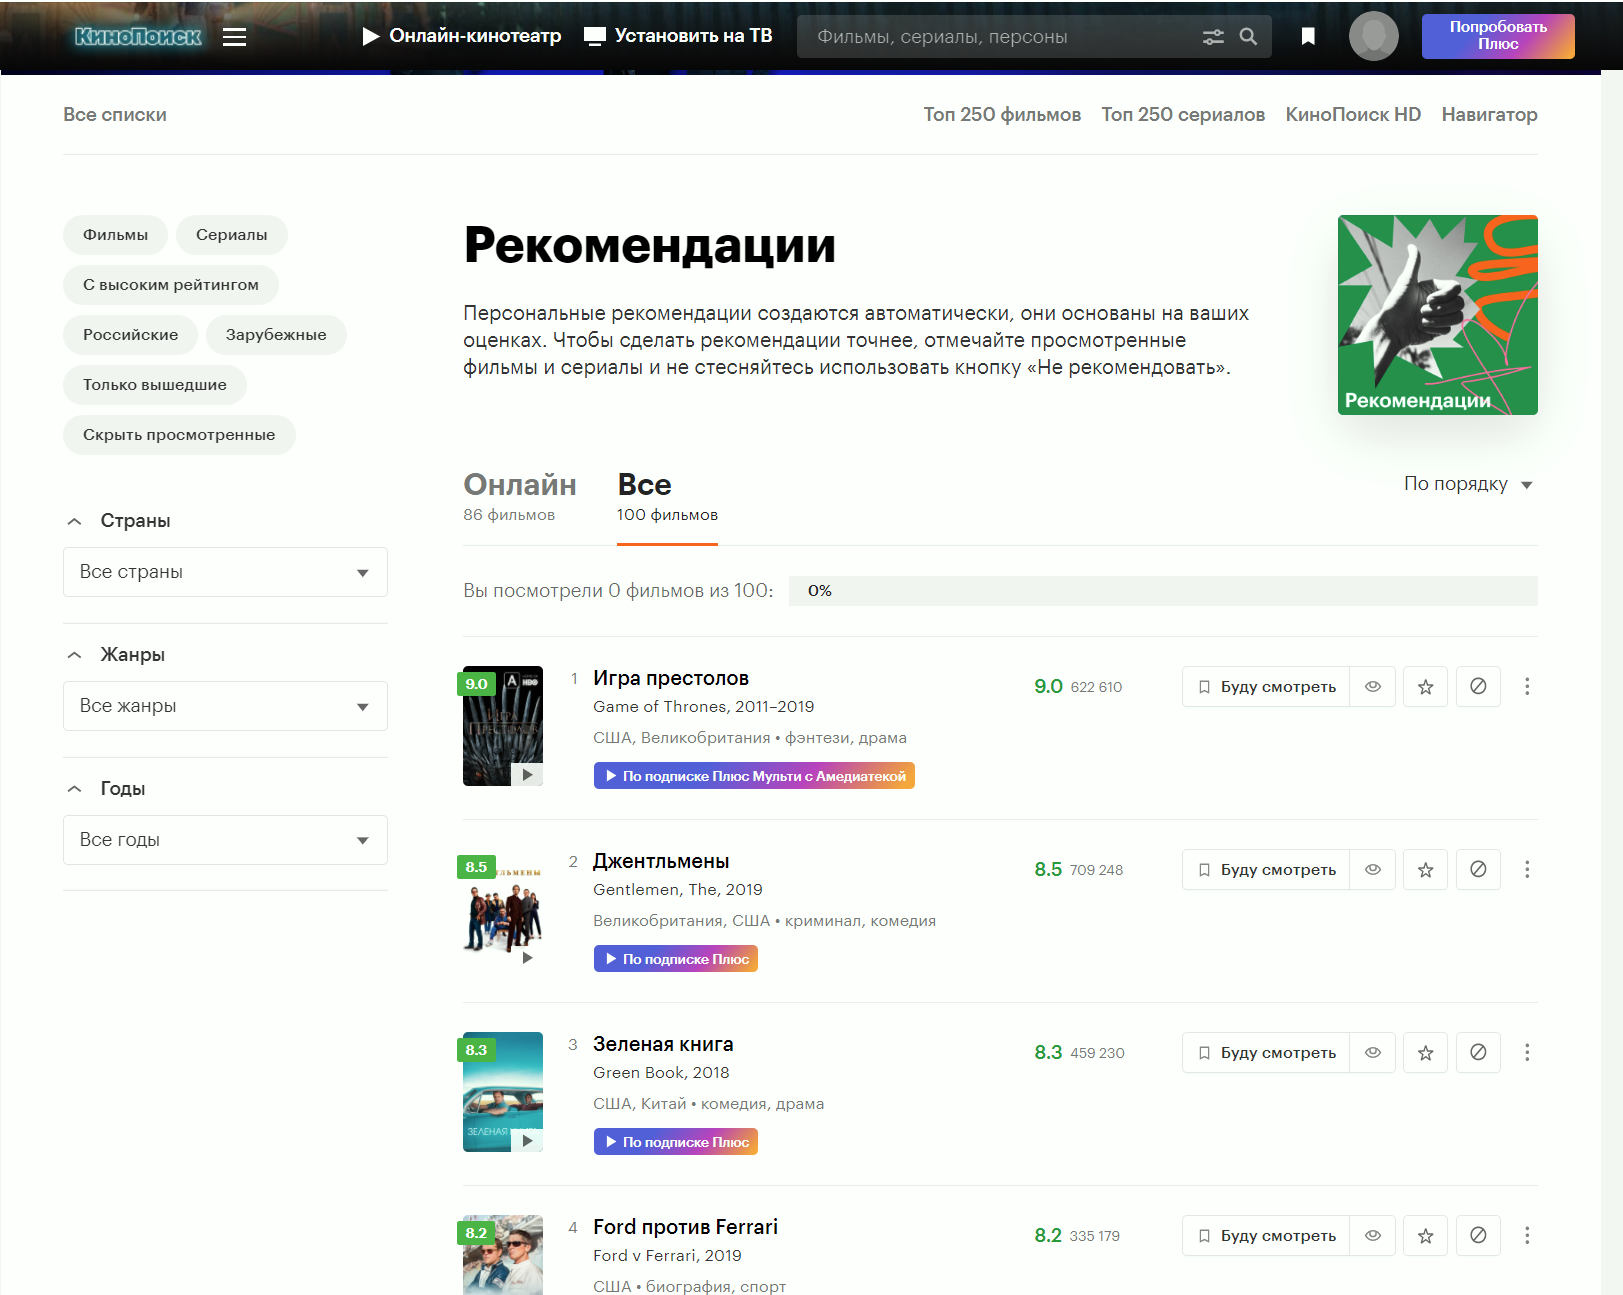
\includegraphics[scale=0.5]{img/kinopoisk.png}
	\caption{Раздел рекомендаций сервиса <<Кинопоиск>>.}
	\label{img:kinopoisk}
\end{figure}  

\newpage
\subsubsection{Аудио-сервисы}
Помимо распространенных кино-сервисов существует великое множество сервисов по подборке музыки: <<Spotify>>, <<Яндекс.Музыка>>, <<Boom>> и другие. Данные сервисы предоставляют для прослушивания музыку разных жанров и от разных исполнителей. Однако, каждый из них имеет систему рекомендаций и всячески старается подчеркнуть ее наличие. У аудио-сервисов рекомендации основаны на добавленных песнях, на любимых исполнителях и жанрах, на прослушанном материале. Ниже на Рисунке \ref{img:Spotify} продемонстрирован внешний вид данного раздела рекомендаций в приложении <<Spotify>>.

\begin{figure}[h!]
	\centering
	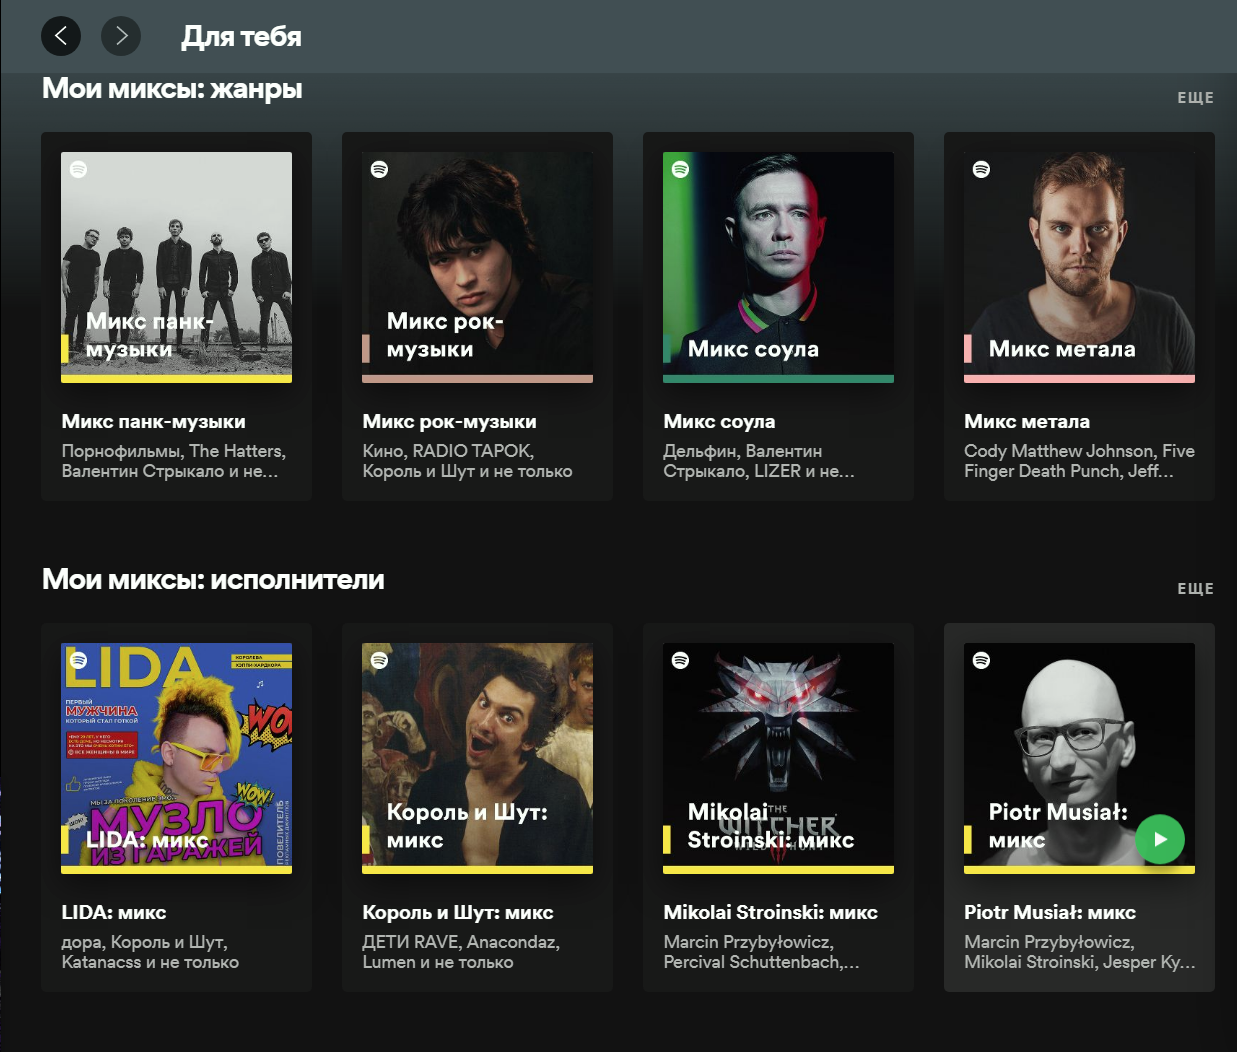
\includegraphics[scale=0.5]{img/spotify.png}
	\caption{Раздел рекомендаций сервиса <<Spotify>>.}
	\label{img:Spotify}
\end{figure}  
\newpage

\subsubsection{Вывод}
Просмотрев популярные медиа-сервисы, приходит понимание, что кино-сервисам не хватает большой и разнообразной системы рекомендаций, основанной на широком спектре интересов пользователя, что присутствует во многих аудио-сервисах.

\subsection{Анализ моделей баз данных}
Модель базы данных - это тип модели данных, которая определяет логическую структуру базы данных и в корне определяет, каким образом данные могут храниться, организовываться и обрабатываться\cite{modelDB}.

\subsubsection{Иерархическая база данных}
Иерархические базы данных имеют форму деревьев с дугами-связями и узлами-элементами данных. Иерархическая структура предполагала неравноправие между данными – одни жестко подчинены другим\cite{modelDB}.

Иерархические базы данных — самая ранняя модель представления сложной структуры данных. Информация в иерархической базе организована по принципу древовидной структуры, в виде отношений «предок-потомок». Каждая запись может иметь не более одной родительской записи и несколько подчиненных. Связи записей реализуются в виде физических указателей с одной записи на другую. Основной недостаток иерархической структуры базы данных — невозможность реализовать отношения «много-ко-многим», а также ситуации, когда запись имеет несколько предков\cite{modelDB}.

\subsubsection{Сетевая модель базы данных}
В сетевых БД наряду с вертикальными реализованы и горизонтальные связи. Однако унаследованы многие недостатки иерархической и главный из них, необходимость четко определять на физическом уровне связи данных и столь же четко следовать этой структуре связей при запросах к базе\cite{modelDB}.

Сетевая модель базы данных подразумевает, что у родительского элемента может быть несколько потомков, а у дочернего элемента — несколько предков. Записи в такой модели связаны списками с указателями. 
Сетевая модель позволяет иметь несколько предков и потомков, формирующих решётчатую структуру.
\subsubsection{Реляционная модель базы данных}
В реляционной модели, в отличие от иерархической или сетевой, не существует физических отношений. Вся информация хранится в виде таблиц (отношений), состоящих из рядов и столбцов. А данные двух таблиц связаны общими столбцами, а не физическими ссылками или указателями. Для манипуляций с рядами данных существуют специальные операторы.

Реляционные таблицы обладают следующими свойствами:
\begin{itemize}
	\item[1)] все значения атомарны;
	\item[2)] каждый ряд уникален;
	\item[3)] порядок столбцов не важен;
	\item[4)] порядок рядов не важен;
	\item[5)] у каждого столбца есть своё уникальное имя.
\end{itemize}

\subsubsection{Выбор модели данных}
 Реляционная модель была выбрана в качестве модели данных. Ее структура данных однозначно определена, не является быстроизменяющейся и данные подчиняются строгим правилам и ограничениям.
\subsection{Анализ СУБД}
СУБД — комплекс программ, позволяющих создать базу данных (БД) и манипулировать данными (вставлять, обновлять, удалять и выбирать). Одними из самых популярных реляционных систем управления базами данных сейчас являются MSSQL, MySQL, PostgreSQL, Oracle.
\subsubsection{MySQL}
MySQL — реляционная СУБД с открытым исходным кодом, главными плюсами которой являются ее скорость и гибкость, которая обеспечена поддержкой большого количества различных типов таблиц.

Преимущества:
\begin{itemize}
	\item[1)] простота в использовании;
	\item[2)] масштабируемость;
	\item[3)] безопасность;
	\item[4)] обширный функционал;
	\item[5)] скорость.    
\end{itemize}
Недостатки:
\begin{itemize}
	\item[1)] недостаточная надежность;
	\item[2)] низкая скорость разработки. 
\end{itemize}
\subsubsection{Microsoft SQL Server}
Система позволяет синхронизироваться с другими программными продуктами компании Microsoft, а также обеспечивает надежную защиту данных и простой интерфейс, однако отличается высокой стоимостью лицензии и повышенным потреблением ресурсов.

Преимущества:
\begin{itemize}
	\item[1)] простота в использовании;
	\item[2)] масштабируемость;
	\item[3)] возможность интеграции с другими продуктами Microsoft.  
\end{itemize}
Недостатки:
\begin{itemize}
	\item[1)] высокая стоимость продукта для юридических лиц; 
	\item[2)] высокая ресурсоемкость SQL Server.  
\end{itemize}
\subsubsection{PostgreSQL}
PostgreSQL — это популярная свободная объектно-реляционная система управления базами данных. PostgreSQL базируется на языке SQL и поддерживает многочисленные возможности.

Преимущества:
\begin{itemize}
	\item[1)] бесплатное ПО с открытым исходным кодом;
	\item[2)] активная поддержка сообщества;
	\item[3)] расширяемость;   
\end{itemize}
Недостатки:
\begin{itemize}
	\item[1)] производительность;

\end{itemize}
\subsubsection{Oracle}
Oracle – это объектно-реляционная система управления базами данных.

Преимущества:
\begin{itemize}
	\item[1)] поддержка огромных баз данных;
	\item[2)] быстрая обработка транзакций;
	\item[3)] большой и постоянно развивающийся функционал.   
\end{itemize}
Недостатки:
\begin{itemize}
	\item[1)] высокая стоимость; 
	\item[2)] значительные вычислительные ресурсы. 
\end{itemize}

\subsection{Вывод}
В данном разделе была поставлена задача, рассмотрены возможные пользователи системы, представлены и проанализированы современные решения, проведен анализ модели данных и СУБД.


%КОНСТРУКТОРСКИЙ РАЗДЕЛ
\clearpage
\section{Конструкторский раздел}
В данном разделе будут рассмотрены сценарии пользователей, спроектирована база данных, описана ролевая модель и спроектировано приложение.
\subsection{Сценарии пользователей}
Нужно определить возможности каждого из видов пользователей. 
\subsubsection{Гость}
Гость — это неавторизованный пользователь, обладающий минимальным набором возможностей взаимодействия с системой. Он может авторизоваться, просмотреть общий список фильмов, актеров, жанров с информацией о них. На Рисунке \ref{img:UseCaseGuest} представлена Use-Case-диаграмма для гостя.

\begin{figure}[h!]
	\centering
	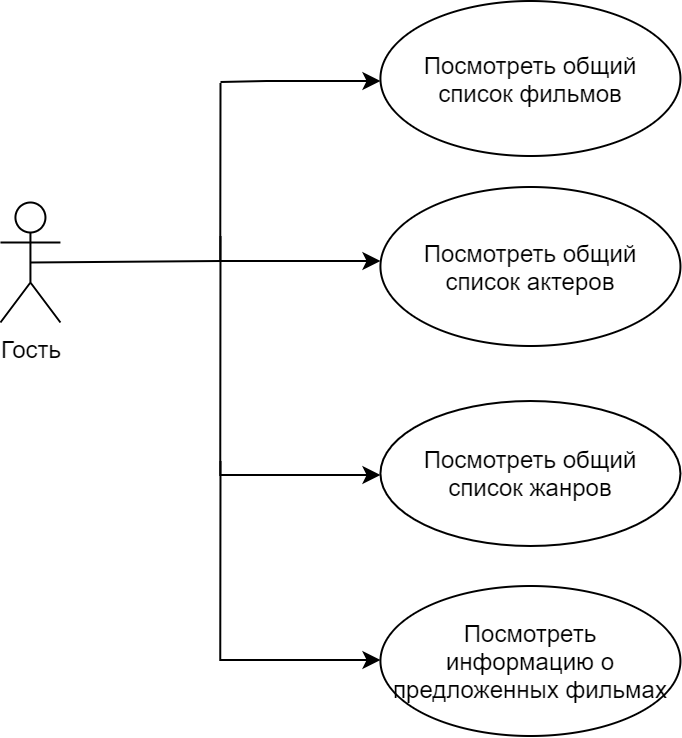
\includegraphics[scale=0.3]{img/UseCaseGuest.png}
	\caption{Сценарии для гостя.}
	\label{img:UseCaseGuest}
\end{figure}
\newpage

\subsubsection{Авторизованный пользователь}
Авторизованному пользователю доступно:
\begin{itemize}
	\item[1)] просмотр общего списка фильмов;
	\item[2)] просмотр общего списка актеров;
	\item[3)] просмотр общего списка жанров;
	\item[4)] добавление/удаление любимых актеров;
	\item[5)] добавление/удаление любимых жанров;
	\item[6)] просмотр информации о рекомендованных фильмах.    
\end{itemize}

На Рисунке \ref{img:UseCaseUser} представлена Use-Case-диаграмма для пользователя.
\begin{figure}[h!]
	\centering
	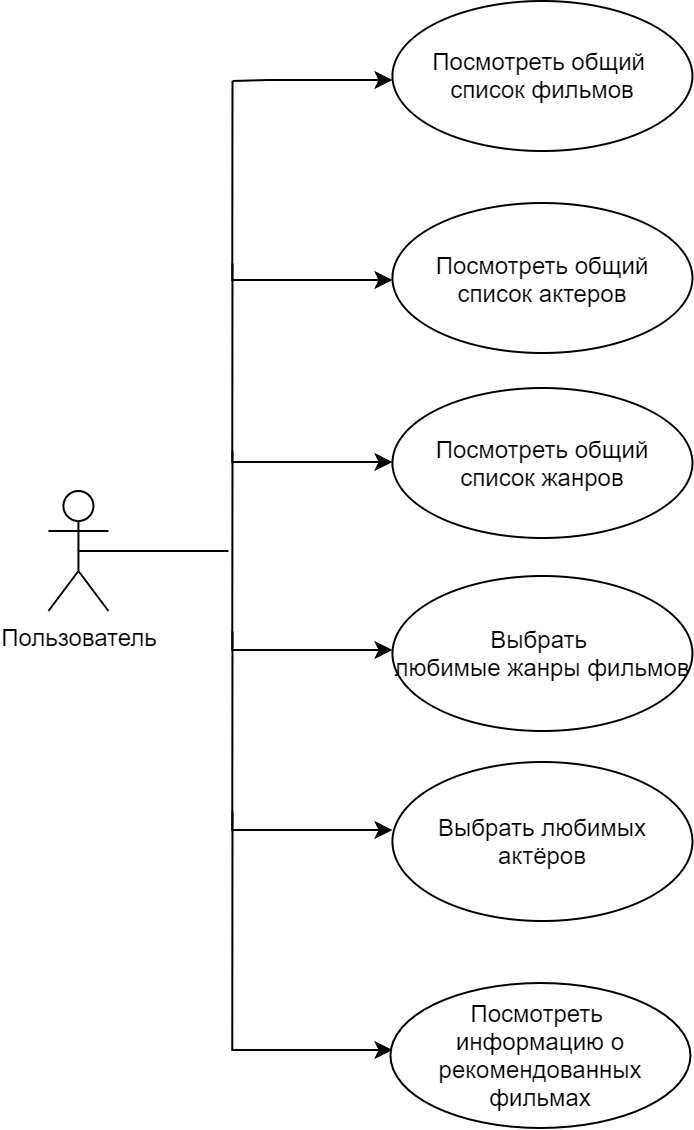
\includegraphics[scale=0.3]{img/UseCaseUser.png}
	\caption{Сценарии для пользователя.}
	\label{img:UseCaseUser}
\end{figure}
\newpage

\subsubsection{Администратор}
Администратору доступно:
\begin{itemize}
	\item[1)] просмотр общего списка студий, фильмов, актеров, жанров, режиссеров, пользователей;
	\item[2)] добавление/удаление фильмов;
	\item[3)] добавление/удаление актёров;
	\item[4)] добавление/удаление жанров;
	\item[5)] добавление/удаление режиссёров;
	\item[6)] добавление/удаление пользователей;
	\item[7)] добавление/удаление студий.  
\end{itemize}
На Рисунке \ref{img:UseCaseAdmin} представлена Use-Case-диаграмма для администратора.
\begin{figure}[h!]
	\centering
	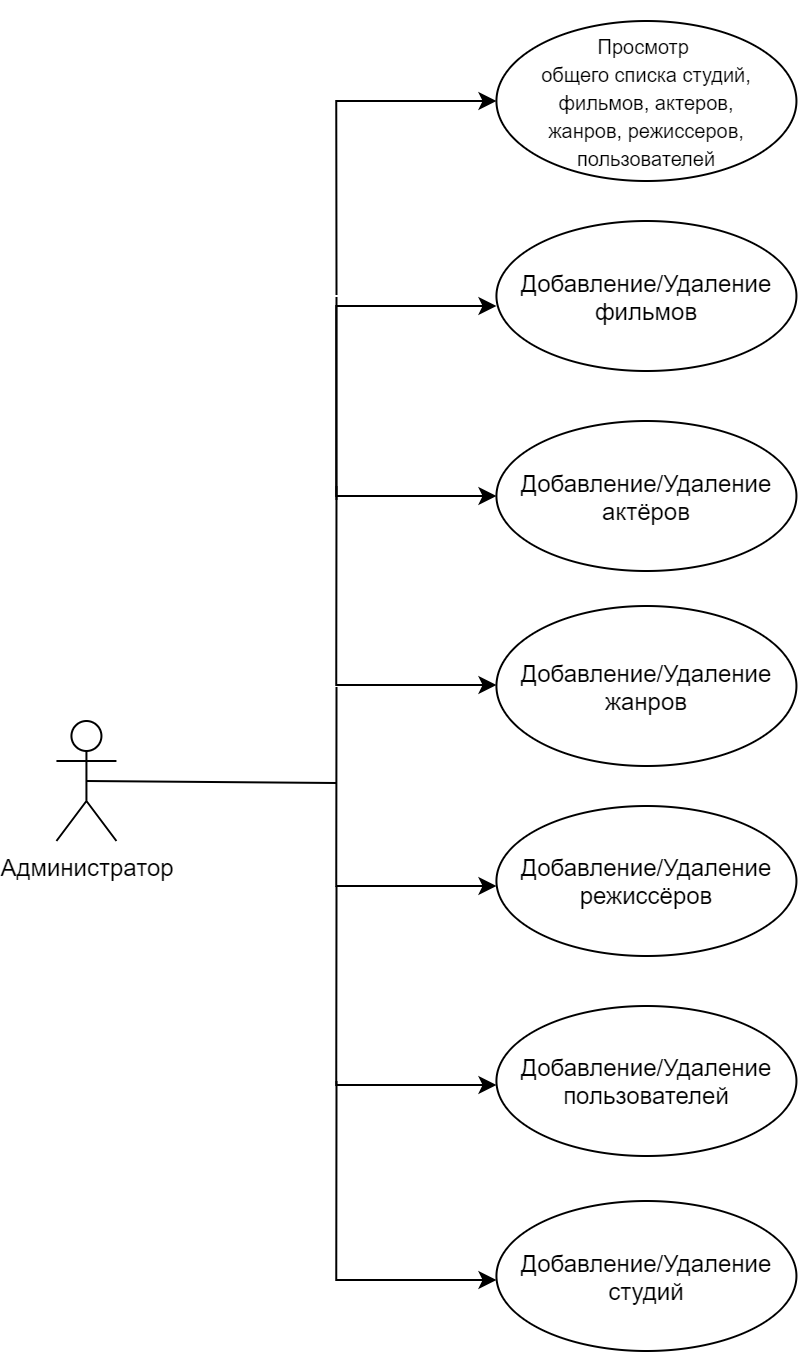
\includegraphics[scale=0.3]{img/UseCaseAdmin.png}
	\caption{Сценарии для администратора.}
	\label{img:UseCaseAdmin}
\end{figure}
\newpage


\subsection{Ролевая модель}
На уровне базы данных выделена следующая ролевая модель:
\begin{itemize}
	\item[1)] guest - гость;
	\item[2)] common\_user - пользователь;
	\item[3)] admin - администратор.  
\end{itemize}
Использование ролевой модели на уровне базы данных гарантирует безопасность доступа к объектам базы данных.

\subsubsection{Гость}
Пользователь с ролью guest имеет следующие права: SELECT над таблицами films, actors, genres, users.

\subsubsection{Пользователь}
Пользователь с ролью common\_user имеет следующие права:
\begin{itemize}
	\item[1)] SELECT над всеми таблицами;
	\item[2)] SELECT, UPDATE, DELETE, INSERT над таблицами любимых жанров и
	 актеров пользователя - user\_genres, user\_actors.    
\end{itemize}

\subsubsection{Администратор}
Пользователь с ролью admin обладает всеми правами.

\subsection{Проектирование базы данных}
\subsubsection{Формализация сущностей системы}
Необходимо выделить сущности предметной области и построить ER-диаграмму. 
На рисунке \ref{img:ER} представлена ER-диаграмма системы.
\begin{figure}[h!]
	\centering
	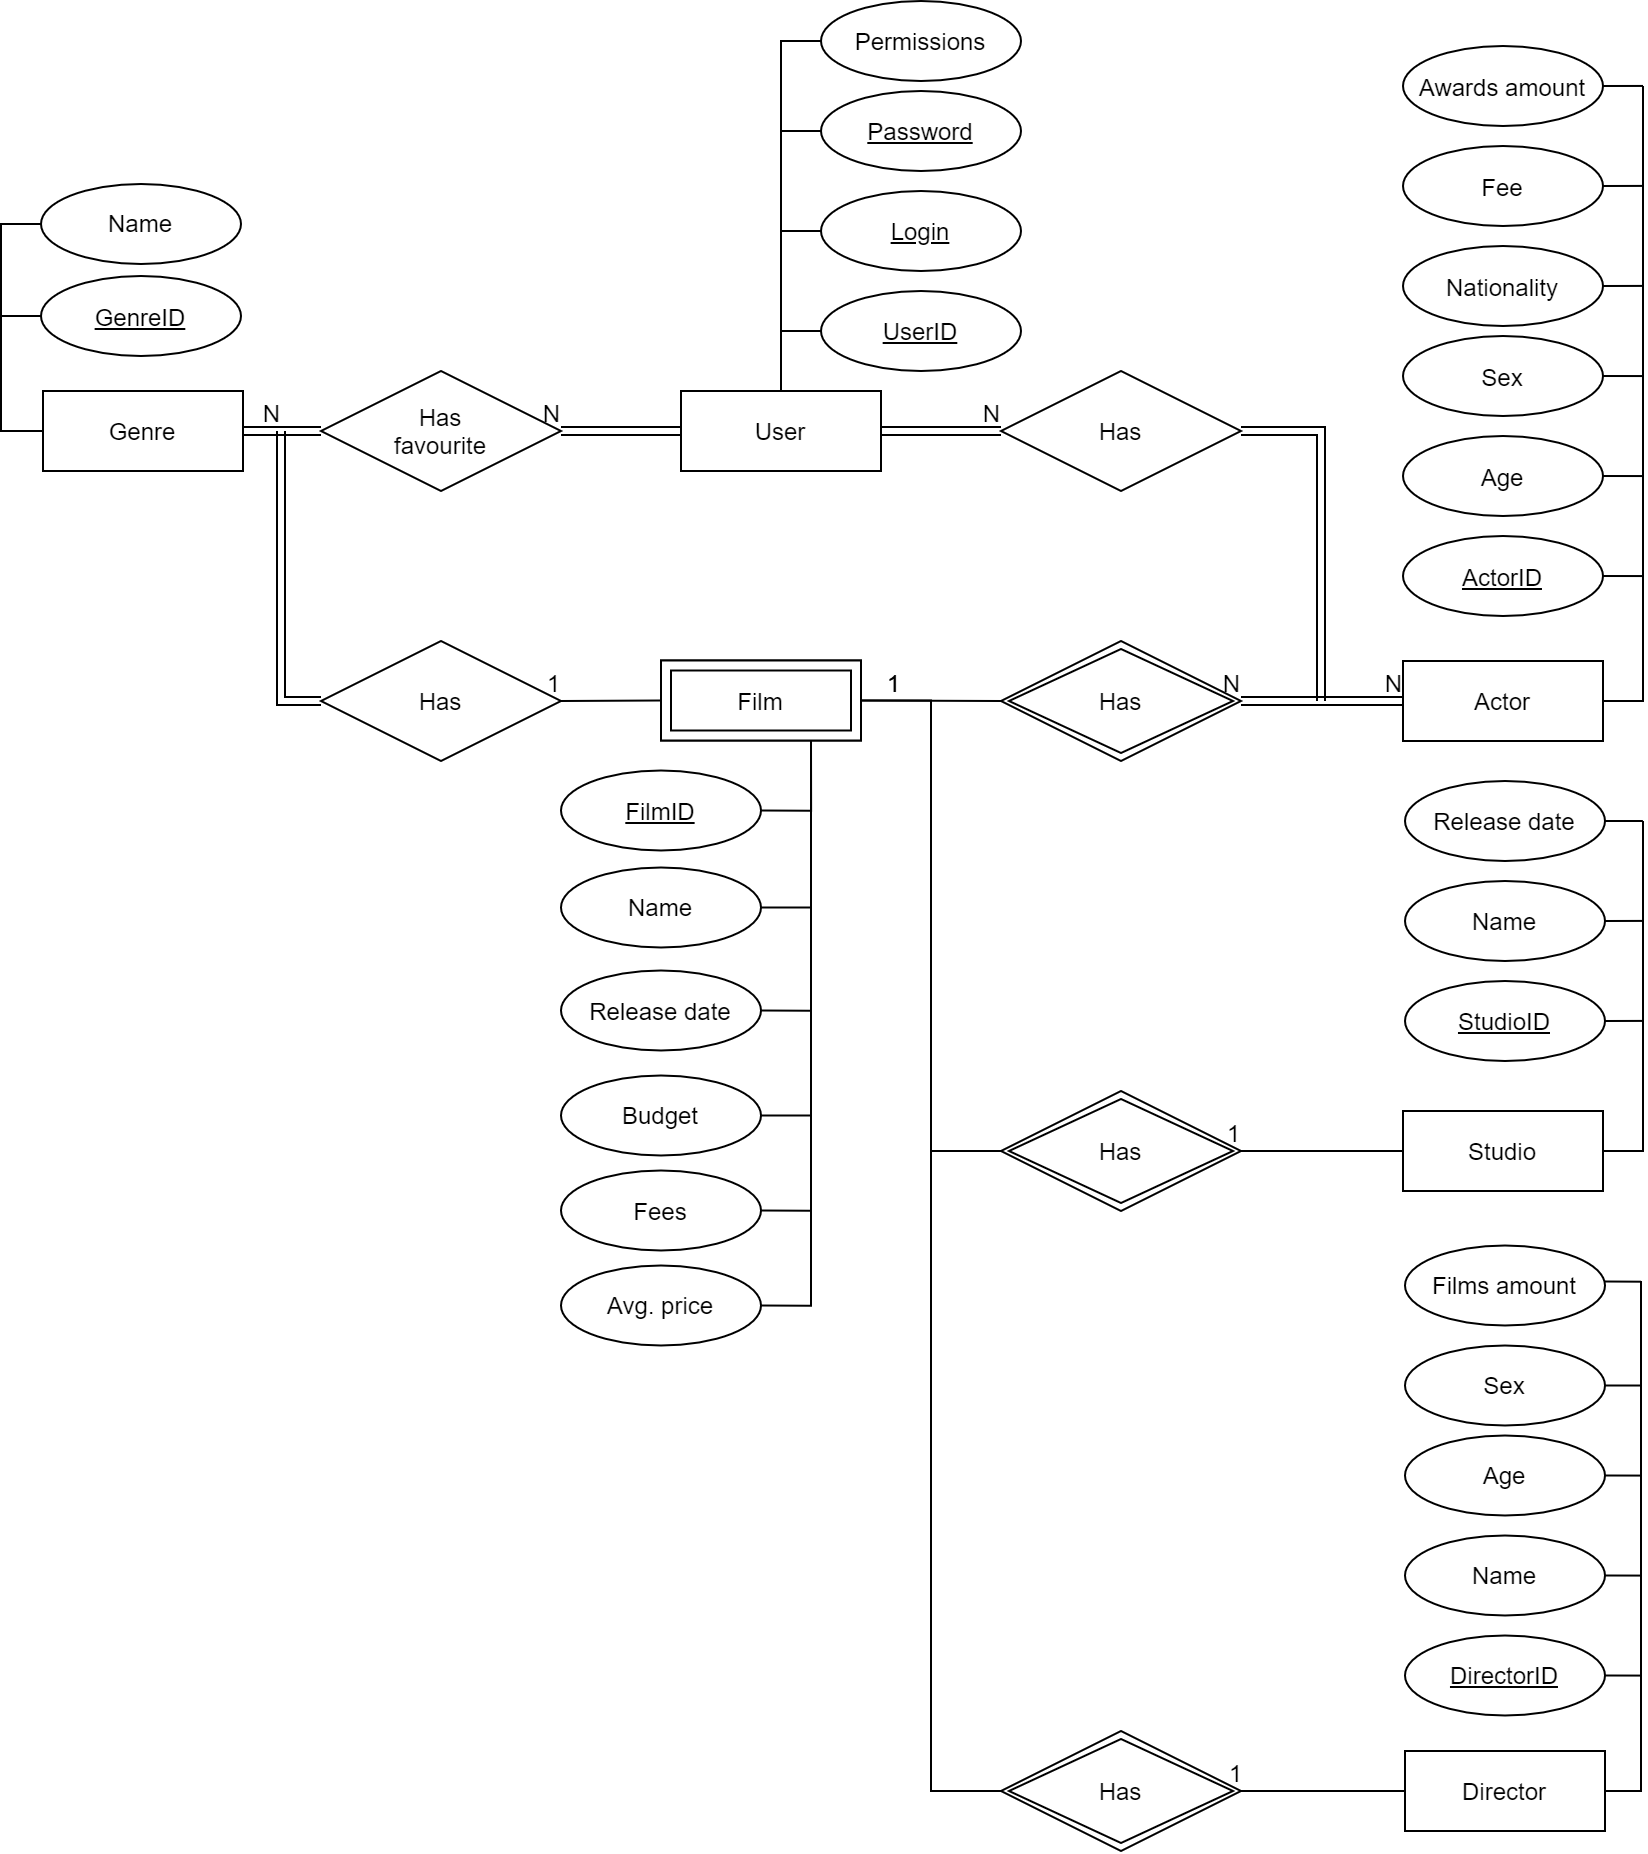
\includegraphics[scale=0.25]{img/ER.png}
	\caption{ER-диаграмма системы.}
	\label{img:ER}
\end{figure}
\newpage

\textbf{Выделенные сущности:}
\begin{itemize}
	\item[1)] Film - таблица, в которой хранится информация о фильмах;
	\item[2)] Actor - таблица, в которой хранится информация об актерах;
	\item[3)] User - таблица, в которой хранится информация о пользователях;
	\item[4)] Genre - таблица, в которой хранится информация о жанрах;
	\item[5)] Studio - таблица, в которой хранится информация о студиях;
	\item[6)] Director - таблица, в которой хранится информация о режиссерах;
\end{itemize}

\subsubsection{Функции}
Для того, чтобы пользователь мог получать рекомендации по фильмам, необходимо добавить функцию, которая возвращает список фильмов, которые могут заинтересовать пользователя, и информацию о них.

\subsection{Проектирование приложения}
В качестве реализации проекта выбрано Desktop-приложение. Оно спроектировано по паттерну MVC. Выделены два компонента - доступа к данным и бизнес-логики. Компонент доступа к данным спроектирован по паттерну <<Репозиторий>>. Для контроля ролей при авторизации пользователя создан класс Connection, в котором обрабатывается конфигурационный файл и возвращается строка подключения. 
\subsection{Вывод}
В данном разделе были рассмотрены сценарии пользователей, спроектирована база данных, описана ролевая модель и спроектировано приложение.

\newpage
%ТЕХНОЛОГИЧЕСКИЙ РАЗДЕЛ
\section{Технологический раздел}
В данном разделе описаны средства реализации поставленной задачи, создание базы данных и ролевая модель, разработаны компоненты и описан порядок работы.

\subsection{Средства реализации поставленной задачи}
Для данного проекта в качестве СУБД была выбрана PostgreSQL\cite{psql}, так как данная система выигрывает по многим параметрам:
\begin{itemize}
	\item[1)] бесплатное ПО с открытым исходным кодом;
	\item[2)] активная поддержка сообщества;
	\item[3)] расширяемость;   
\end{itemize}

В качестве языка программирования был выбран язык C\#\cite{sharp}, так как:
\begin{itemize}
	\item[1)] имеются удобные пакеты для работы с PostgreSQL;
	\item[2)] ООП язык программирования, что позволяет использовать наследование, интерфейсы, абстракции и т.п.
\end{itemize}

В качестве среды разработки была выбрана <<Microsoft Visual Studio 2019>>\cite{vs}, так как:
\begin{itemize}
	\item[1)] имеет удобный интерфейс для написания отладки кода;
	\item[2)] обеспечивает бесплатный доступ для студентов;
	\item[3)] позволяет работать с Windows Forms\cite{wf}.  
\end{itemize}
Для работы с базой данных был выбран Entity Framework\cite{efcore}, так как EF Core поддерживает запросы LINQ, отслеживание изменений, обновления и миграции схемы и работает с многими базами данных, включая PostgreSQL.

\subsection{Создание базы данных}
Требуется построить диаграмму БД по выделенным сущностям. В приложении А приведен листинг создания таблиц БД. На Рисунке \ref{img:DB} представлена диаграмма БД. 
\begin{figure}[h!]
	\centering
	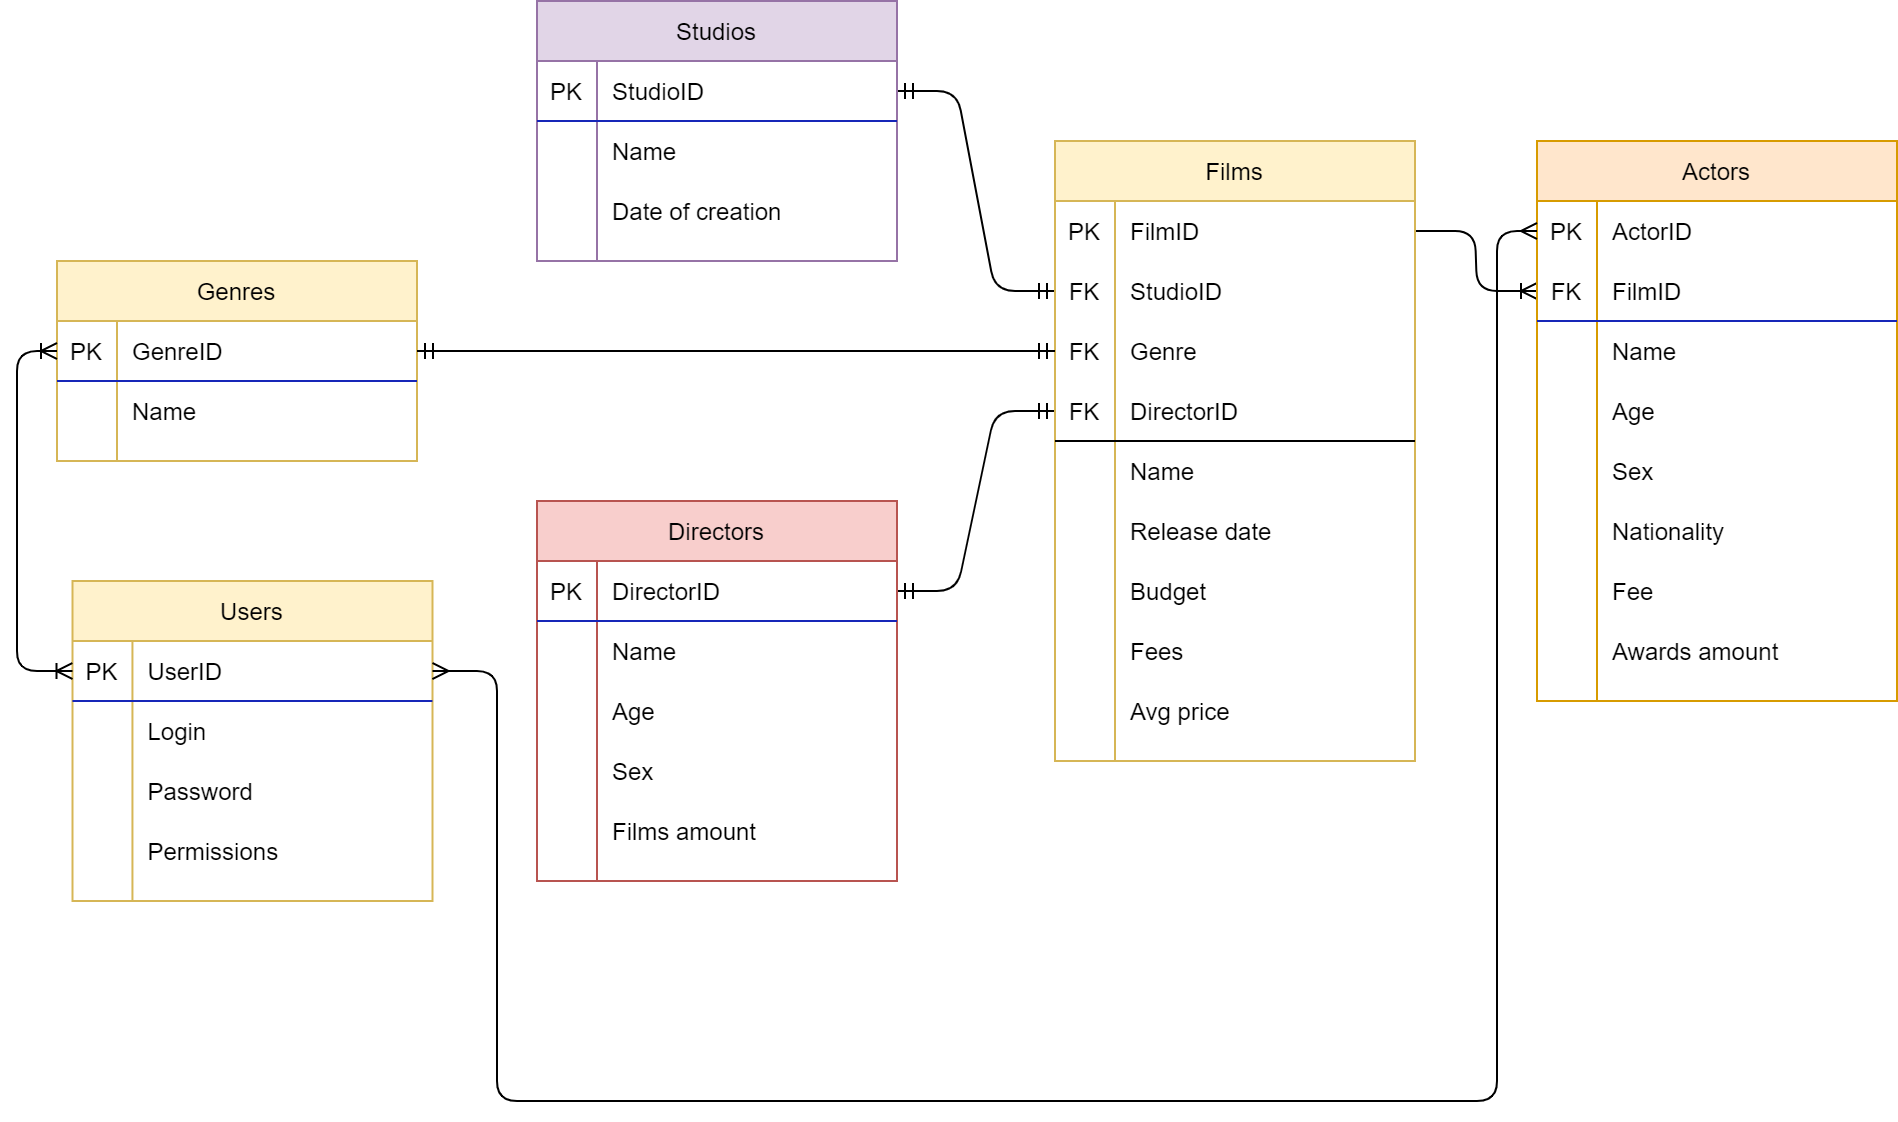
\includegraphics[scale=0.25]{img/DB.png}
	\caption{Диаграмма БД.}
	\label{img:DB}
\end{figure}
\newpage

\subsection{Функции}
В Листинге \ref{lst:func} представлена реализация функции get\_recommended\_films.
\begin{lstlisting}[label={lst:func},caption=Реализация функции GetPlayers., language=SQL]
create or replace function get_recommended_films(int)
returns table
(
	film_name varchar(40),
	release_date date,
	budget int,
	fees int,
	avg_price int
)
language sql
as $$
	select film_name, release_date, budget, fees, avg_price
	from users join user_actors
	on $1 = user_actors.user_id
	join actors on actors.actor_id = user_actors.actor_id
	join films on films.film_id = actors.film_id
	union
	select film_name, release_date, budget, fees, avg_price
	from users join user_genres
	on $1 = user_genres.user_id
	join genres on genres.genre_id = user_genres.genre_id
	join films on films.genre_id = genres.genre_id
$$;
\end{lstlisting}

\subsection{Разработка компонентов}
Приложение спроектировано по паттерну MVC, поэтому следует реализовать компоненты доступа к данным и бизнес-логики.

\subsubsection{Компонент доступа к данным}
На Рисунке \ref{img:AccessToDB} представлена UML-диаграмма компонента доступа к данным.
\begin{figure}[h!]
	\centering
	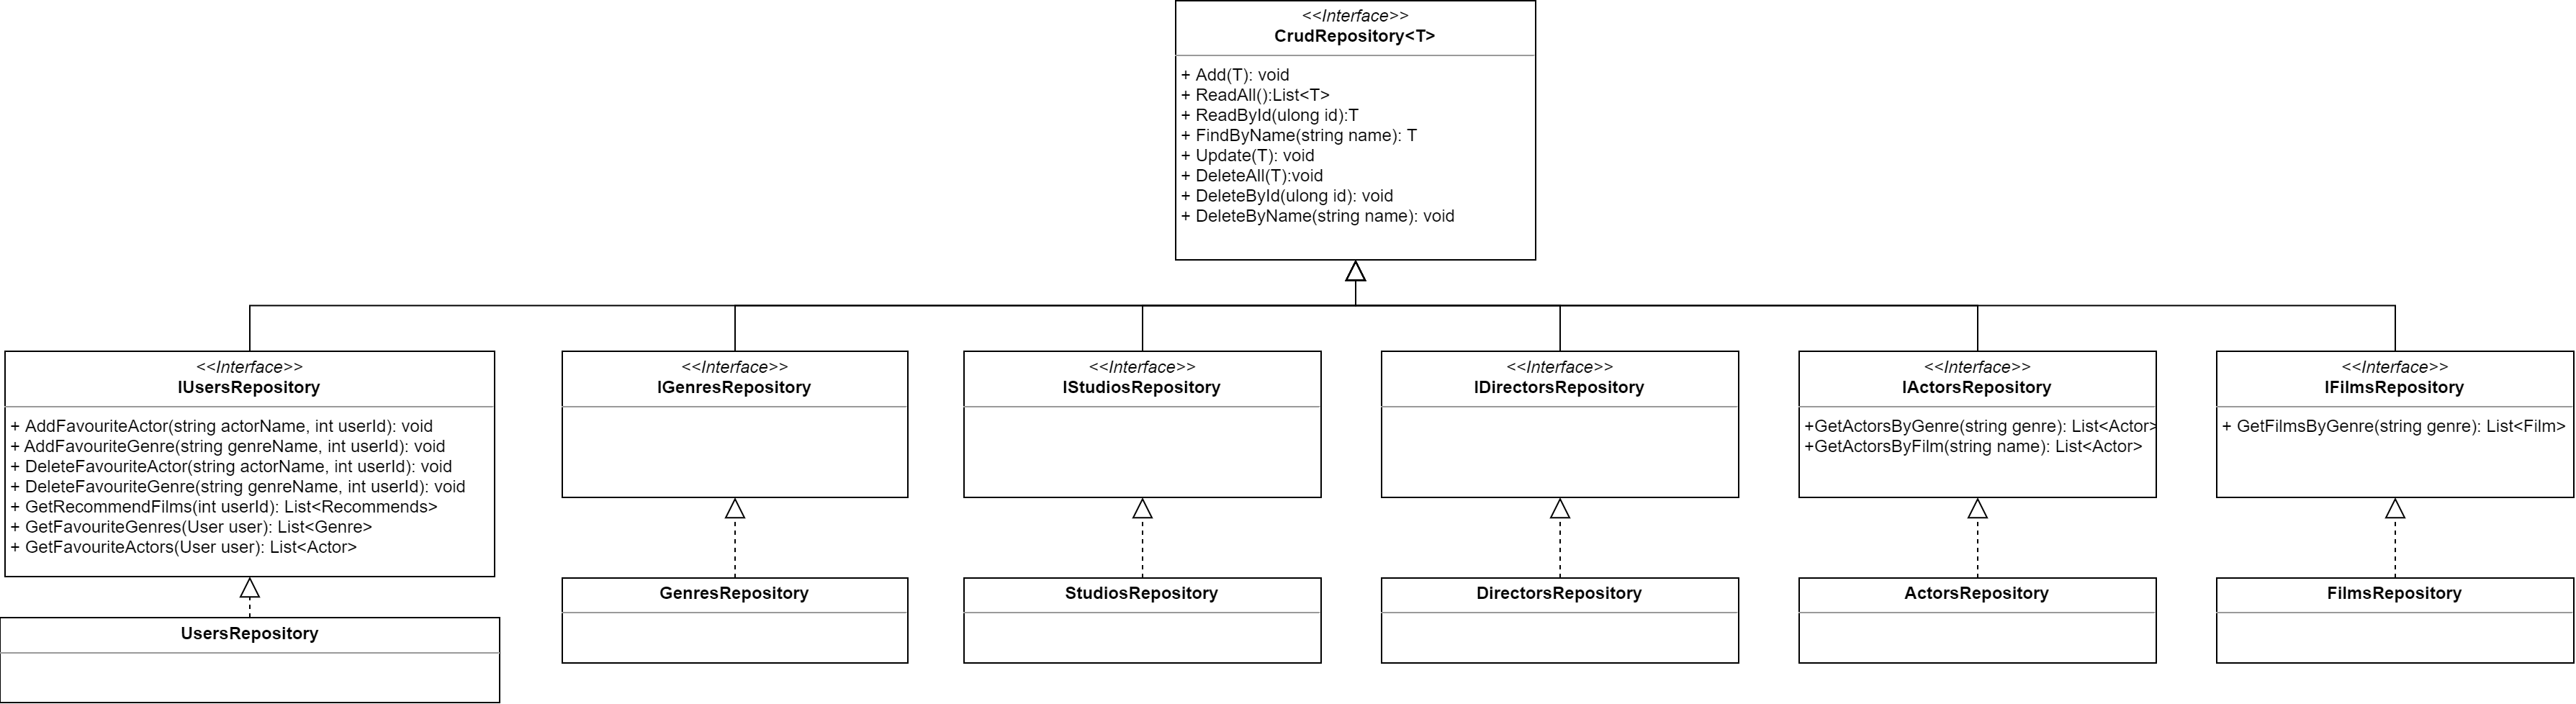
\includegraphics[scale=0.14]{img/AccessToDB.png}
	\caption{Компонент доступа к данным.}
	\label{img:AccessToDB}
\end{figure}

\subsubsection{Компонент бизнес-логики}
На Рисунке \ref{img:Controllers} представлена UML-диаграмма компонента бизнес-логики.
\begin{figure}[h!]
	\centering
	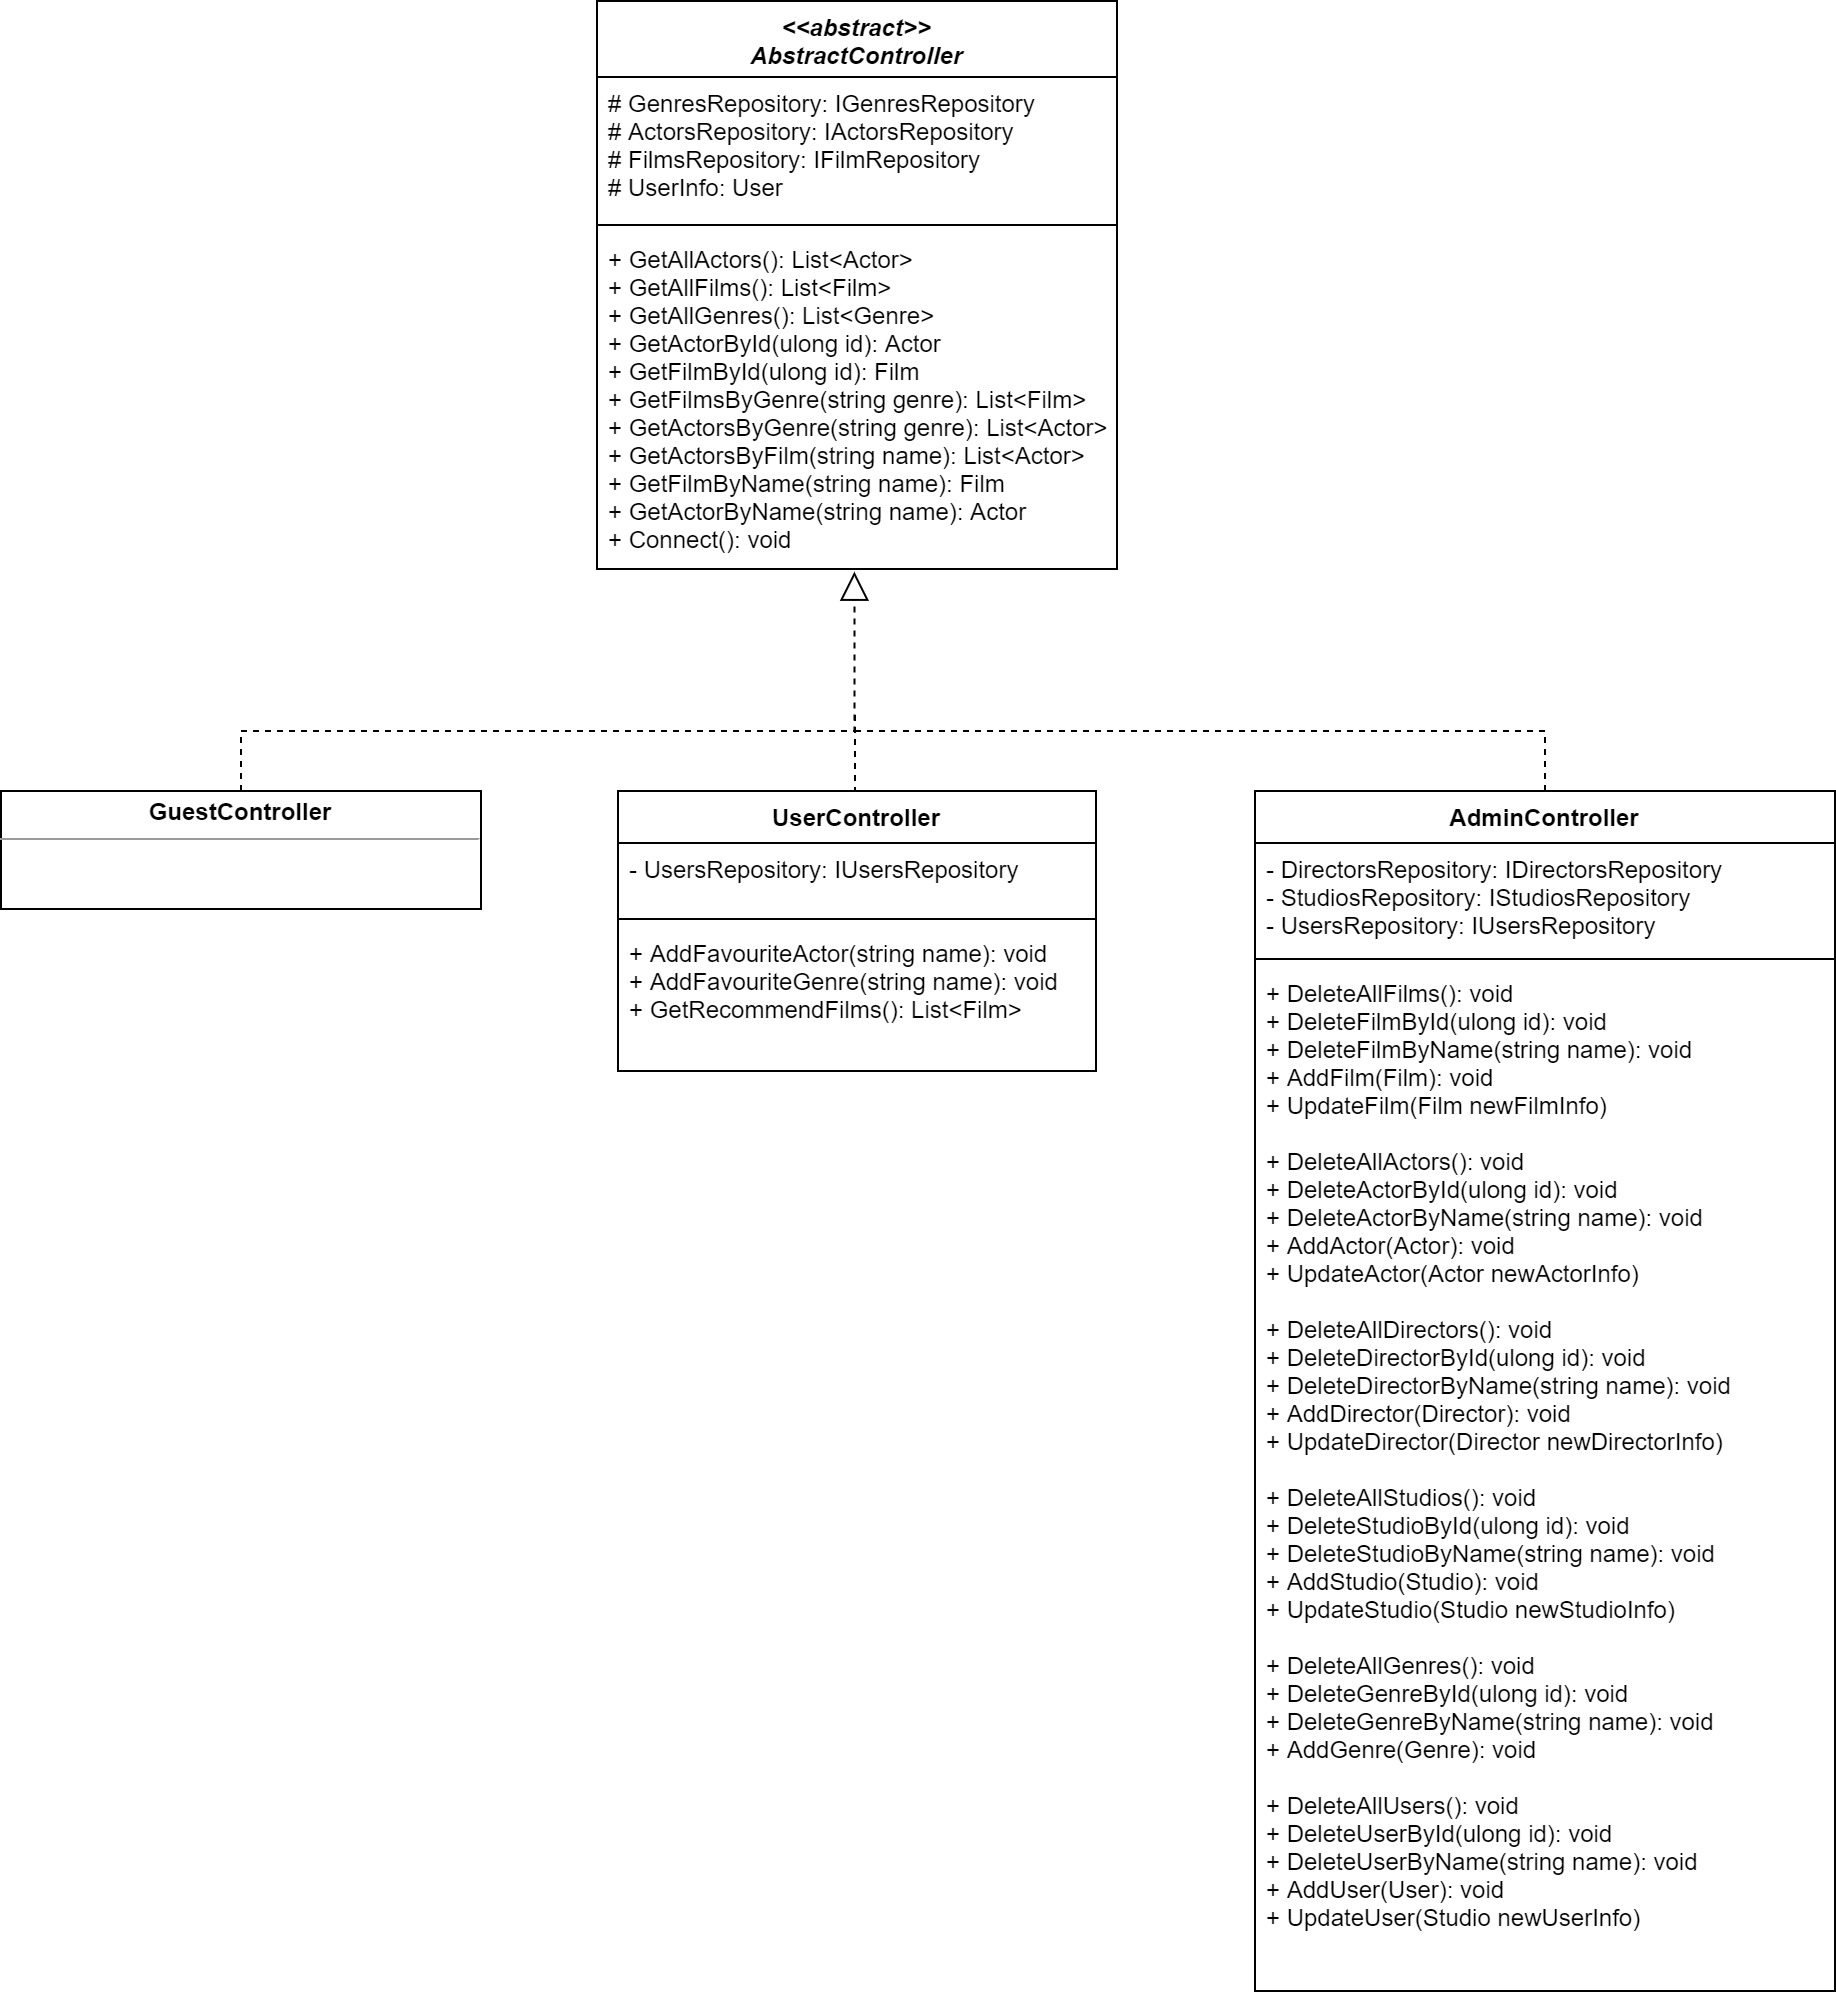
\includegraphics[scale=0.25]{img/Controllers.png}
	\caption{Компонент бизнес-логики.}
	\label{img:Controllers}
\end{figure}
\newpage
\subsection{Интерфейс приложения}
На Рисунках ниже показан интерфейс авторизации и интерфейсы пользователей 
(гость, авторизованный пользователь, администратор).

\begin{figure}[h!]
	\centering
	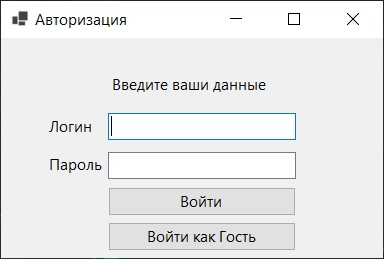
\includegraphics[scale=1]{img/auth.jpg}
	\caption{Окно авторизации.}
	\label{img:auth}
\end{figure}
\begin{figure}[h!]
	\centering
	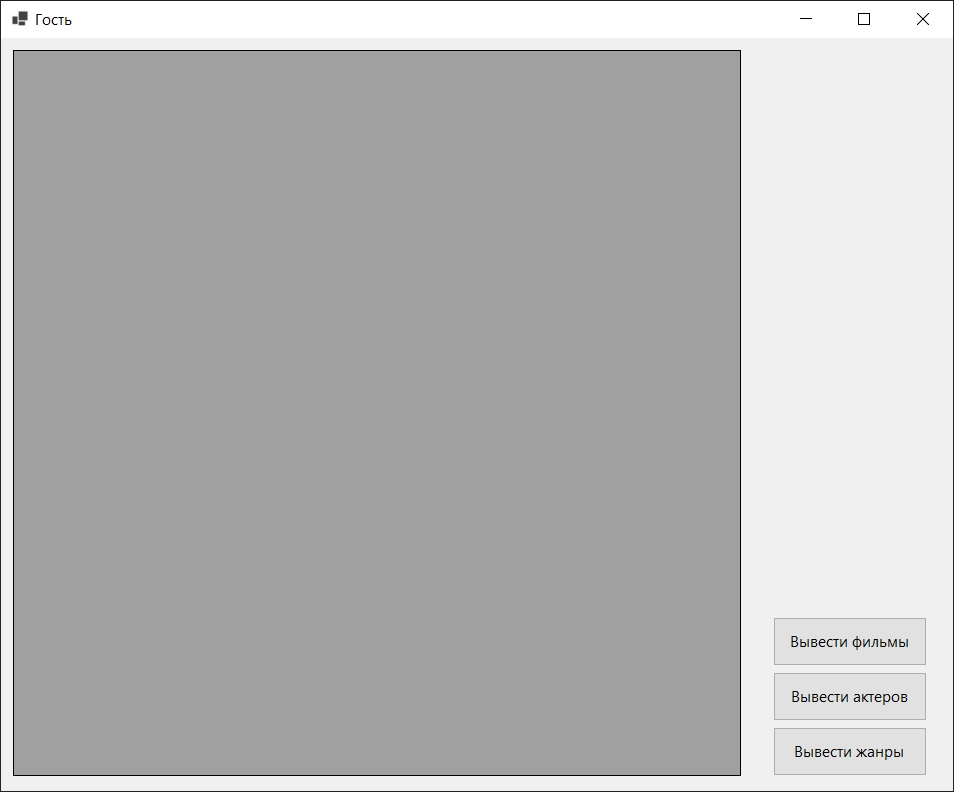
\includegraphics[scale=0.9]{img/guest.jpg}
	\caption{Окно гостя.}
	\label{img:guest}
\end{figure}
\clearpage
\begin{figure}[h!]
	\centering
	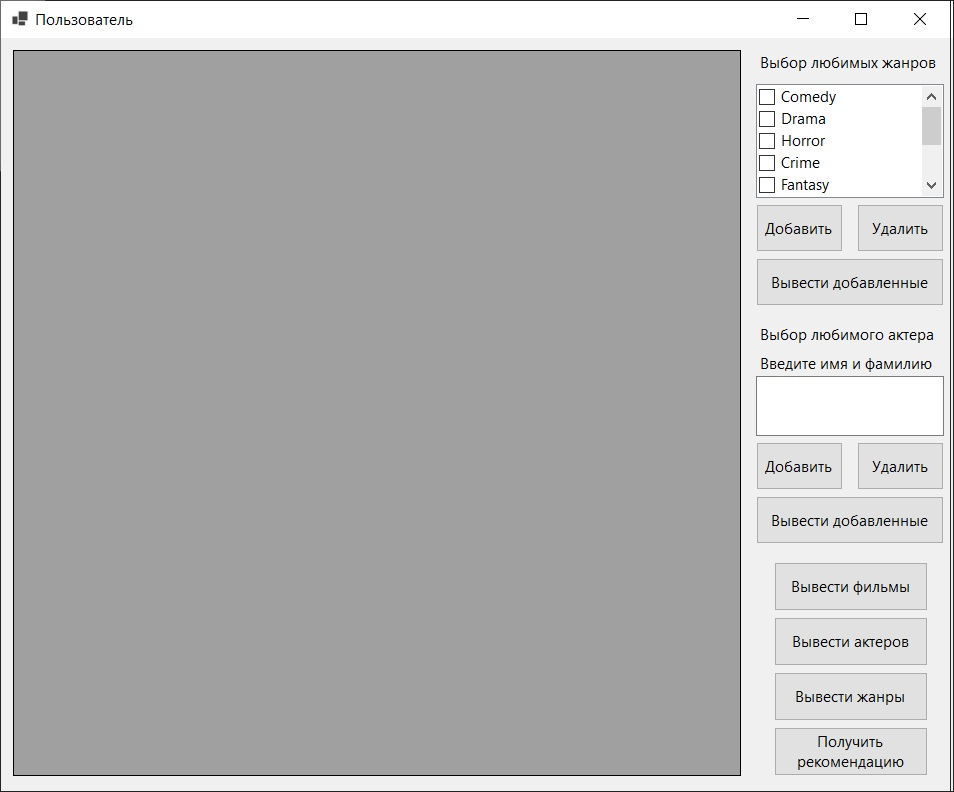
\includegraphics[scale=0.90]{img/user.jpg}
	\caption{Окно авторизованного пользователя.}
	\label{img:user}
\end{figure}
\clearpage
\begin{figure}[h!]
	\centering
	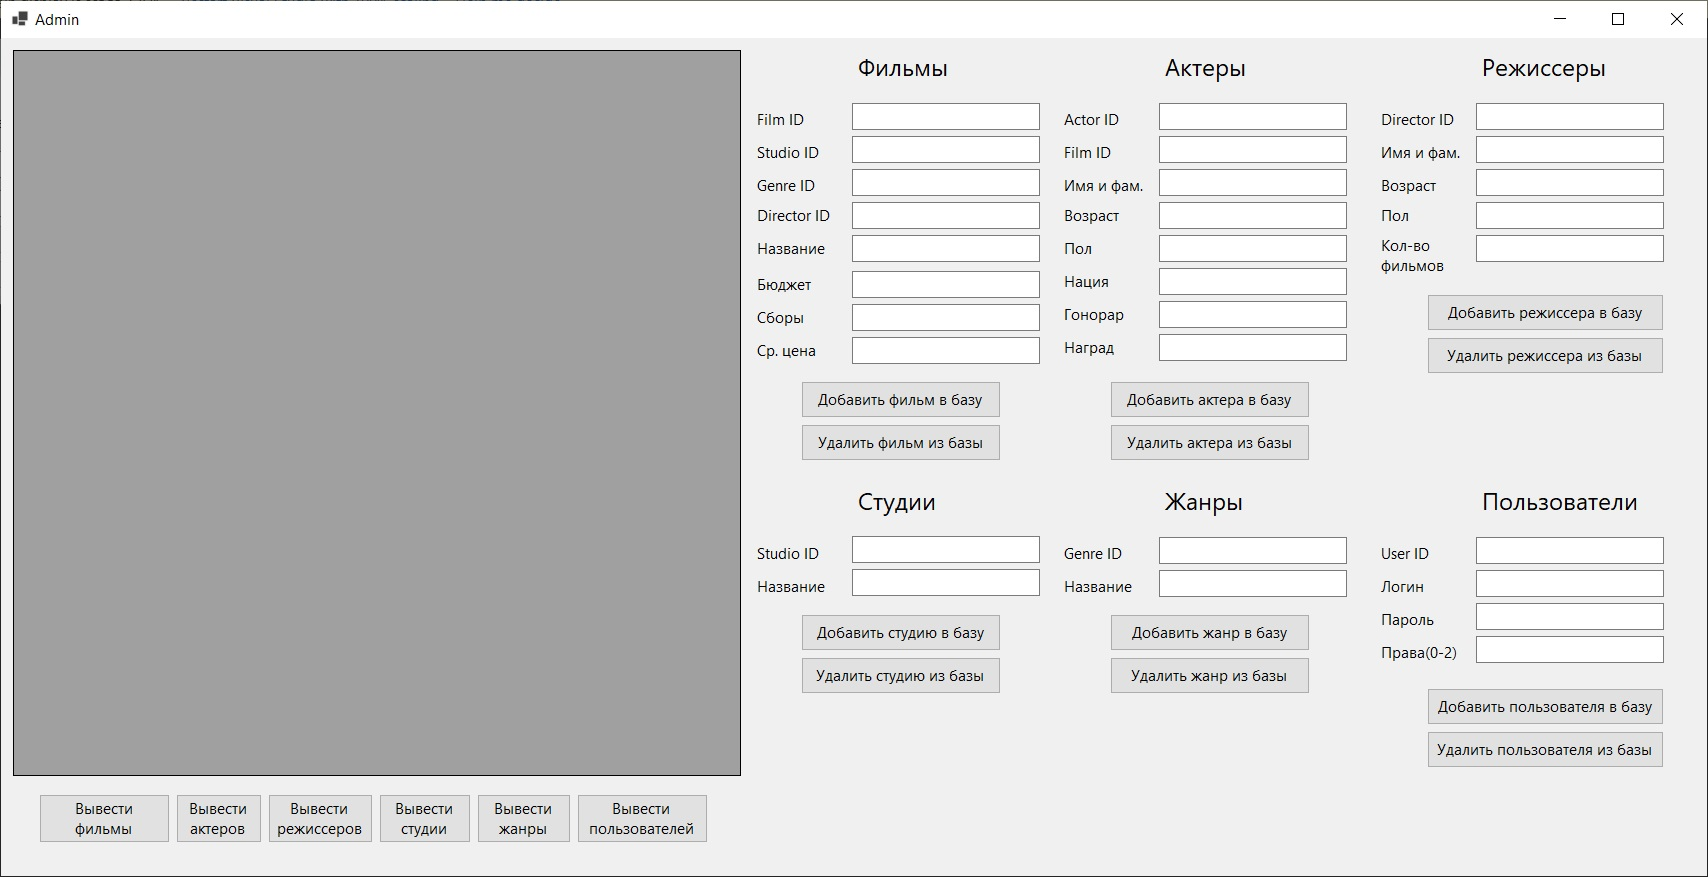
\includegraphics[scale=0.50]{img/admin.jpg}
	\caption{Окно администратора.}
	\label{img:admin}
\end{figure}

\subsection{Вывод}
В данном разделе были выбраны средства реализации поставленной задачи, создана база данных и описана ролевая модель на уровне БД, разработаны компоненты и описан порядок работы.
\newpage
\section*{Заключение}
\addcontentsline{toc}{section}{Заключение}
Цель курсовой работы достигнута.

В ходе выполнения курсовой работы было формализовано задание, выделены соответствующие пользователи и их функционал, проведен анализ и выбор наиболее подходящей для данной задачи СУБД, спроектирована база данных, приложение.

В результате, с использованием языка программирования C\# и СУБД PostgreSQL было создано многофункциональное приложение  для получения информации о фильмах, рекомендованных пользователю. Получен опыт разработки базы данных и приложения по паттерну MVC. 

В дальнейшей перспективе приложение и база данных могут был масштабированы. Может быть добавлен следующий функционал:
\begin{itemize}
	\item[1)] оценки фильмов пользователями и рекомендации на их основе;
	\item[2)] добавление новой информации о фильмах путем новых полей и сущностей;
	\item[3)] добавление пользователя с не такими огромными правами, как у администратора, но способного исполнять его основные обязанности.
\end{itemize}

\clearpage
%СПИСОК ЛИТЕРАТУРЫ
\begin{thebibliography}{9}
	\addcontentsline{toc}{section}{Литература}
	\bibitem{modelDB} Национальная библиотека им. Н. Э. Баумана Bauman National Library : [Электронный ресурс] URL: https://postgrespro.ru/docs/postgresql (дата обращения: 20.05.2021).
	\bibitem{psql} PostgreSQL : Документация [Электронный ресурс] URL: https://postgrespro.ru/docs/postgresql (дата обращения: 20.05.2021).
	\bibitem{sharp} Документация по C\# [Электронный ресурс] URL: https://docs.microsoft.com/ru-ru/dotnet/csharp/ (дата обращения: 20.05.2021).
	\bibitem{vs} Документация по семейству продуктов Visual Studio [Электронный ресурс] URL: https://docs.microsoft.com/ru-ru/visualstudio/?view=vs-2019 (дата обращения: 20.05.2021).
	\bibitem{wf} Windows Forms [Электронный ресурс] URL: https://docs.microsoft.com/ru-ru/dotnet/desktop/winforms/?view=netdesktop-5.0 (дата обращения: 20.05.2021).
	\bibitem{efcore} Документация по Entity Framework [Электронный ресурс] URL: https://docs.microsoft.com/ru-ru/ef/ (дата обращения: 20.05.2021).
\end{thebibliography}
 
\clearpage
{\centering\textbf{Приложение А.} \par}
{\centering Создание таблиц базы данных. \par}
\addcontentsline{toc}{section}{Приложение А. Создание таблиц базы данных.}
\begin{lstlisting}[label={lst:appA}, language=SQL]
create table if not exists studios(
	studio_id int primary key,
	studio_name varchar(40) not null,
	date_of_creation date
);

create table if not exists directors(
director_id int primary key,
director_name varchar(40) not null,
age int check(age > 23 and age < 71),
sex varchar (6),
films_amount int check(films_amount > 0 and films_amount < 10)
);

create table if not exists genres(
	genre_id int primary key,
	genre_name varchar(40)
);

create table if not exists films(
	film_id int primary key,
	studio_id int references studios(studio_id),
	genre_id int references genres(genre_id),
	director_id int references directors(director_id),
	film_name varchar(40) not null,
	release_date date,
	budget int check(budget >= 20000 and budget <= 250000000),
	fees int check(fees >= 20000 and fees <= 1000000000),
	avg_price int check(avg_price >= 120 and avg_price <= 500)
);

create table if not exists actors(
	actor_id int primary key,
	film_id int references films(film_id),
	actor_name varchar(40) not null,
	age int check(age > 17 and age < 71),
	sex varchar(6),
	nationality varchar(40),
	fee int check(fee >= 1000 and fee <= 1000000),
	awards int check(awards >= 0 and awards < 6)
);

create table if not exists users(
	user_id int primary key,
	login varchar(40) not null,
	password varchar(40) not null,
	permissions int 
);

create table if not exists user_genres(
	user_id int references users(user_id),
	genre_id int references genres(genre_id)
);

create table if not exists user_actors(
	user_id int references users(user_id),
	actor_id int references actors(actor_id)
);
\end{lstlisting}

\addcontentsline{toc}{section}{Приложение Б. Презентация.}
\end{document}
